%\title{LaTeX Portrait Poster Template}
%%%%%%%%%%%%%%%%%%%%%%%%%%%%%%%%%%%%%%%%%
% a0poster Portrait Poster
% LaTeX Template
% Version 1.0 (22/06/13)
%
% The a0poster class was created by:
% Gerlinde Kettl and Matthias Weiser (tex@kettl.de)
% 
% Adapter by Jens Buysse for Hogeschool Gent
% This template has been downloaded from:
% http://www.LaTeXTemplates.com
%
% License:
% CC BY-NC-SA 3.0 (http://creativecommons.org/licenses/by-nc-sa/3.0/)
%
%%%%%%%%%%%%%%%%%%%%%%%%%%%%%%%%%%%%%%%%%

%----------------------------------------------------------------------------------------
%	PACKAGES AND OTHER DOCUMENT CONFIGURATIONS
%----------------------------------------------------------------------------------------

\documentclass[a0,portrait]{a0poster}

\usepackage{multicol} % This is so we can have multiple columns of text side-by-side
\columnsep=100pt % This is the amount of white space between the columns in the poster
\columnseprule=3pt % This is the thickness of the black line between the columns in the poster

\usepackage[svgnames]{xcolor} % Specify colors by their 'svgnames', for a full list of all colors available see here: http://www.latextemplates.com/svgnames-colors

\usepackage{times} % Use the times font
%\usepackage{palatino} % Uncomment to use the Palatino font

\usepackage{graphicx} % Required for including images
\graphicspath{{figures/}} % Location of the graphics files
\usepackage{booktabs} % Top and bottom rules for table
\usepackage[font=small,labelfont=bf]{caption} % Required for specifying captions to tables and figures
\usepackage{amsfonts, amsmath, amsthm, amssymb} % For math fonts, symbols and environments

\begin{document}

%----------------------------------------------------------------------------------------
%	POSTER HEADER 
%----------------------------------------------------------------------------------------

% The header is divided into two boxes:
% The first is 75% wide and houses the title, subtitle, names, university/organization and contact information
% The second is 25% wide and houses a logo for your university/organization or a photo of you
% The widths of these boxes can be easily edited to accommodate your content as you see fit

\begin{minipage}[t]{0.75\linewidth}
\VeryHuge \color{HoGentAccent1} \textbf{How will quantum computing affect the mainframe environment and its applications?} \color{Black}\\ % Title
\Huge\textit{2019-2020}\\[2.4cm] % Subtitle
\huge \textbf{Marivoet Lukas, Francis Harkins, Martijn Saelens}\\[0.5cm] % Author(s)
\huge Hogeschool Gent, Valentin Vaerwyckweg 1, 9000 Gent\\[0.4cm] % University/organization
\Large \texttt{lukas.marivoet@student.hogent.be} \\
\end{minipage}
%
\begin{minipage}[t]{0.25\linewidth}

\end{minipage}

\vspace{1cm} % A bit of extra whitespace between the header and poster content

%----------------------------------------------------------------------------------------

\begin{multicols}{2} % This is how many columns your poster will be broken into, a portrait poster is generally split into 2 columns

%----------------------------------------------------------------------------------------
%	ABSTRACT
%----------------------------------------------------------------------------------------

\color{HoGentAccent1} % Navy color for the abstract

\begin{abstract}
	Quantum computing is still in its infancy, but it has already shown off its potential in many different areas. What is important to understand is that together with developing the technology itself, we need to develop the ways we use and interact with this new field. The paper shows an emphasis on the applications of implementing quantum computing in existing sectors. 
\end{abstract}
%----------------------------------------------------------------------------------------
%	INTRODUCTION
%----------------------------------------------------------------------------------------

\color{HoGentAccent1} 
\section*{Introduction}
\color{black}
\color{black}
Why would we already start learning this experimental way of computing? We need to look at quantum computing as an addition to our current systems, the technology combined with our classical way of computing will grant us the ability to simulate drugs, environments etc. to perfect precisions in the long run. It is extremely powerful as a tool because it allows the system to utilise exponentially more data-items compared to a classical device. The exponential factor is gained through the use of superposition and entanglement of qubits, which are both quantum phenomena.
%----------------------------------------------------------------------------------------
%	GEOLOGY
%----------------------------------------------------------------------------------------

\color{Black} % DarkSlateGray color for the rest of the content
\color{HoGentAccent1} 
\section*{Experiment}
\color{black}
We have chosen for an adaptation of an algorithm that could prove extremely useful for
any implementation combined with a mainframe, for example the Grover Search algorithm
applied to the boolean satisfiability problem. The experiment has been created through the use of Qiskit, which is an open-source tool created by IBM for writing your own quantum circuits. The algorithm itself was executed on a real quantum device from IBMQ.

\color{black}


\begin{center}\vspace{1cm}
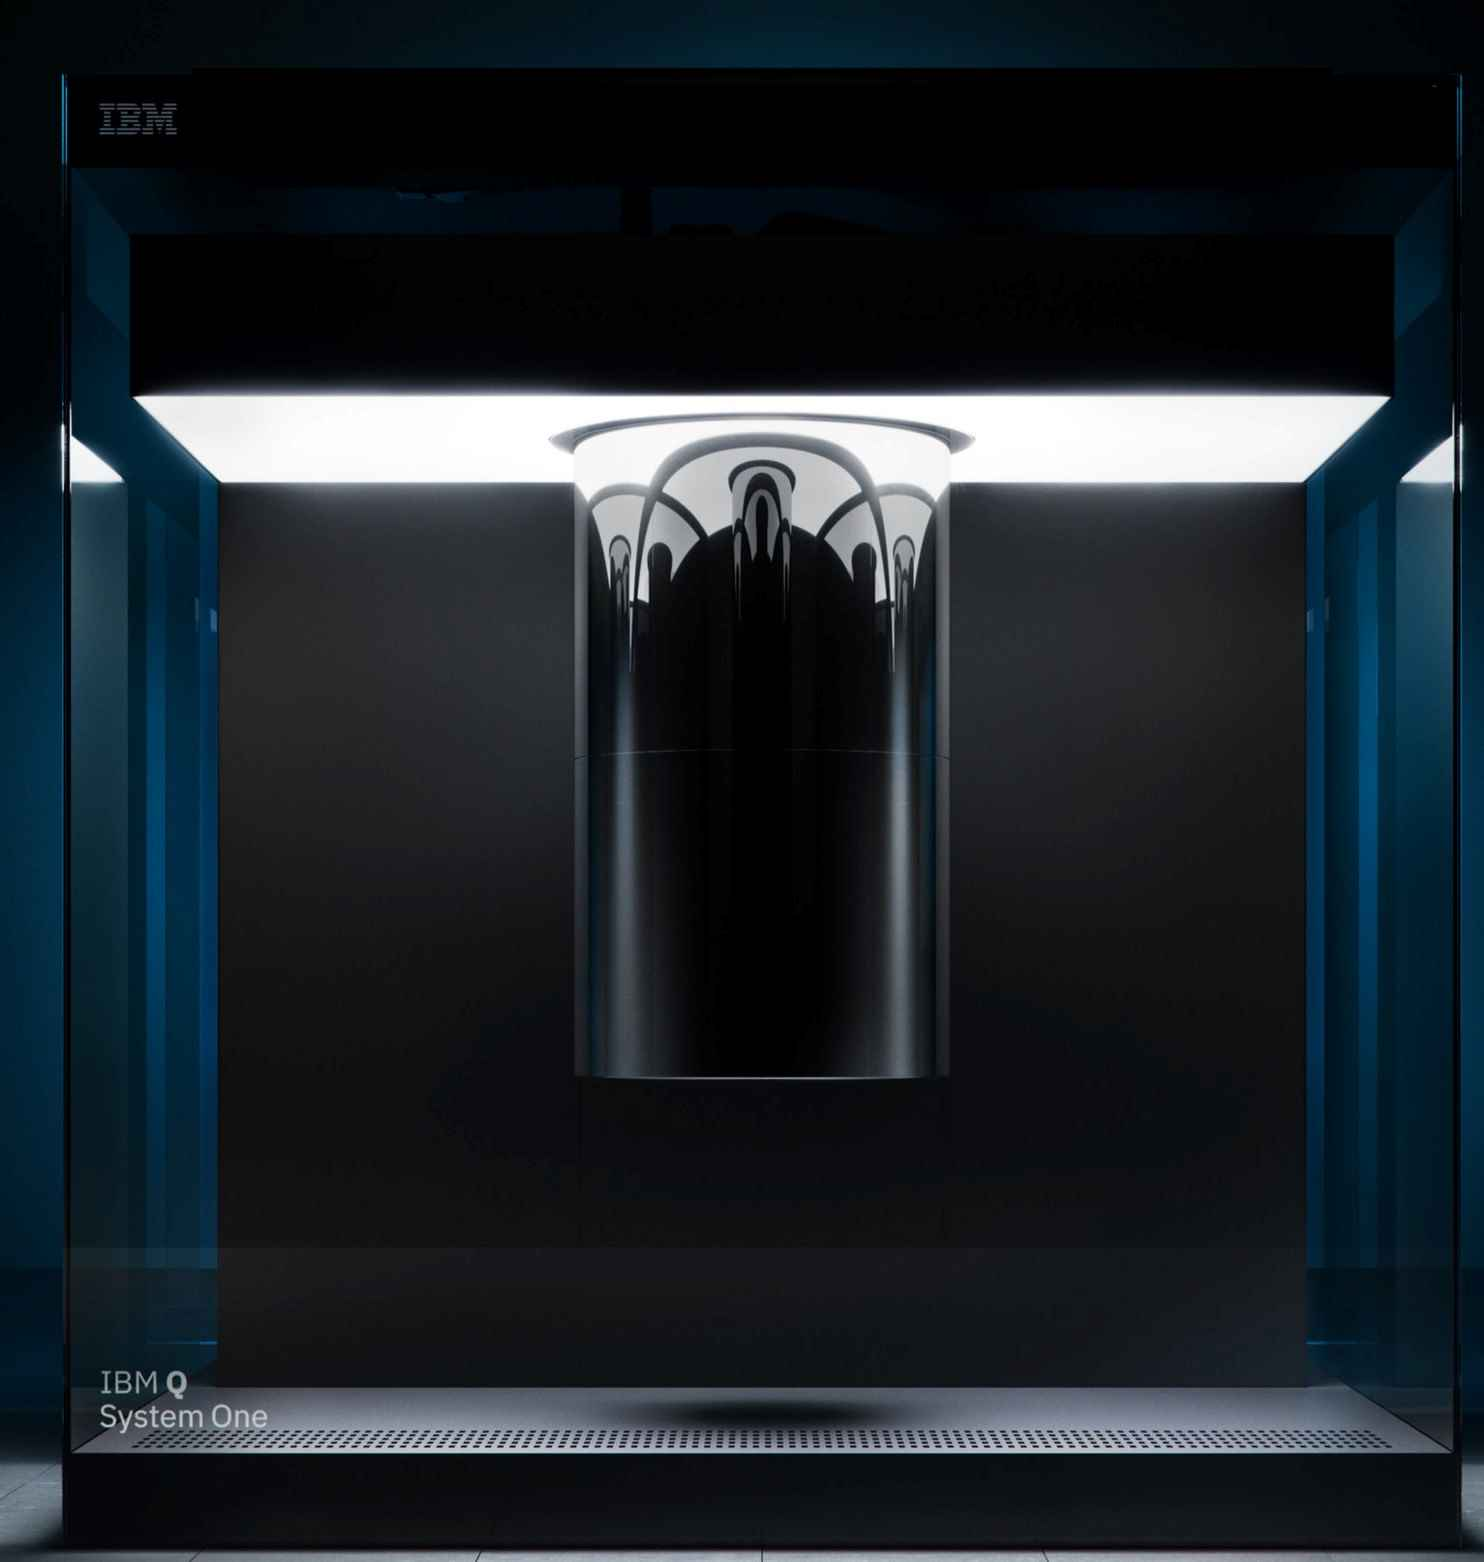
\includegraphics[width=0.5\linewidth]{QCTest}
\end{center}\vspace{1cm}


\color{HoGentAccent1} 
\section*{Conclusions}
\color{black}
The experiment has shown the clear weaknesses of quantum computing at this point in time.

Firstly it has shown how quantum decoherence influences the whole environment too much to provide its necessary reliable results. Secondly we have found out that data-encoding is a giant hurdle to overcome. Mainframes rely on a high amount of classical data, which means that quantum computing as of now, can not provide reliable and valuable results to any mainframe device. It takes too long to encode our classical data for the quantum device, which makes the whole process not viable with any currently available system.

Developing the software for these quantum devices was completely open-source and through the utilisation of Qiskit it became clear that anybody interested in the subject could easily try out their first experiments. So go for it and write your own quantum program today using tools like Qiskit!
%----------------------------------------------------------------------------------------
%	FORTHCOMING RESEARCH
%----------------------------------------------------------------------------------------
\color{HoGentAccent1} 
\section*{Future research}
\color{black}

The potential powerhouse of a mainframe device and a quantum computer can still prove
to be advantageous in future works. If IBM keeps up with doubling its pace of releasing
quantum computational resources into the world each year, there may be a chance that
mainframes and QC prove to be viable in the near future. Also quantum error correction
needs to evolve to an acceptable percentage to where we could start thinking about
implementing QC machine learning algorithms in our mainframes or even the speeding up
the database structures in the devices by using algorithms like Grover’s. But for now QC
and mainframe are not able to cooperate in an useful manner to add more business value.


%----------------------------------------------------------------------------------------

\end{multicols}
\end{document}